\documentclass[12pt]{article}
\usepackage{amsmath,latexsym,amsfonts,amssymb,graphicx,amsthm,epsfig,enumerate}
\usepackage{tikz,verbatim,tabularx} % adds charting fuctions
\newcolumntype{C}{>{\centering\arraybackslash}X}
\linespread{1.2}

%\pagestyle{empty}

\begin{document}
	\title{6 Man's Morris: 2AA4/2ME3 Assignment 2} %add title here
	\author{
		Gregory Smilski, 1404091\\
		Abigail Gaulin, 1327924\\
		Karl Knopf 1437217} 
	% add other necessary information here
	
	\maketitle
	\thispagestyle{empty}
	\newpage
	\tableofcontents
	\newpage
	
	\section{Introduction}
	This document describes the java project 6 Men's Morris. 
	\subsection{Architecture}
	\begin{figure}[!h]
		\centering
		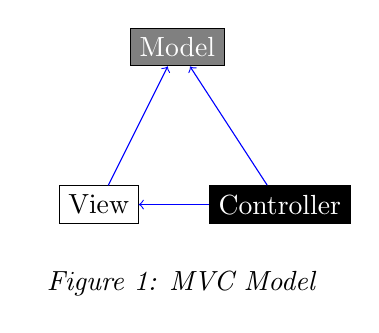
\begin{tikzpicture}
		% MVC Architecture
		\node[draw] (View) at (0,0) {View};
		\node[draw,fill=black,text=white] (Controller) at (2.3,0) {Controller};
		\node[draw,fill=gray,text=white] (Model) at (1,2) {Model};
		
		\draw[->,draw=blue] (View) to (Model);
		\draw[->,draw=blue] (Controller) to (View);
		\draw[->,draw=blue] (Controller) to (Model);
		\node at (1.0, -1.0) {\textit{ Figure 1: MVC Model}};
		
		\end{tikzpicture}
	\end{figure}
	This software uses MVC architecture in its design. MVC stands for Model, View, Controller, and is a design tool used in software development. The View contains all information the user sees, and interacts with the user. The Model contains all the data, and the Controller contains commands which modify the view and model. This architectural style is useful as it allows for modulation, and parts of the program can be modified without affecting any others.
	\subsection{Technologies}
	\begin{itemize}
		\item Java:  An object oriented programming language 
		\item Eclipse: It is an IDE used for the development and testing of software typically in Java
		\item Java Swing: A java toolkit designed to aid programmers in the creation of gui applications. This widget toolkit allows the programmer quick access to various predefined graphical objects, allowing the easy creation of a graphical interface.
		
	\end{itemize}
	\section{Modular Decomposition}
	% 4.1Description of the classes and modules and why they were used
		\begin{figure}[!h]
			\centering
			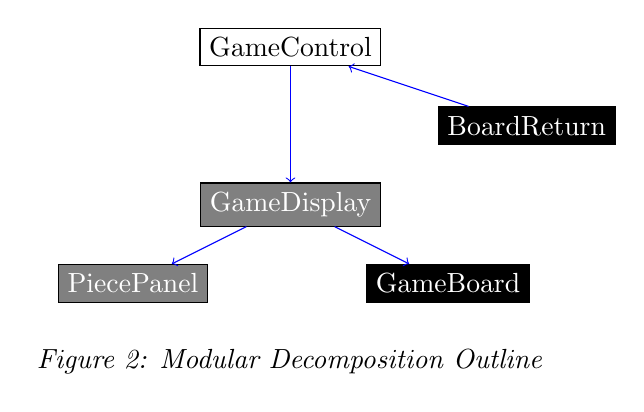
\begin{tikzpicture}
			% MVC Architecture
			\node[draw] (GameControl) at (1,3) {GameControl};
			\node[draw,fill=black,text=white] (GameBoard) at (3,0) {GameBoard};
			\node[draw,fill=gray,text=white] (GameDisplay) at (1,1) {GameDisplay};
			\node[draw,fill=gray,text=white] (PiecePanel) at (-1,0) {PiecePanel};
			\node[draw,fill=black,text=white] (BoardReturn) at (4,2) {BoardReturn};
			
			\draw[->,draw=blue] (GameControl) to (GameDisplay);
			\draw[->,draw=blue] (GameDisplay) to (PiecePanel);
			\draw[->,draw=blue] (GameDisplay) to (GameBoard);
			\draw[->,draw=blue] (BoardReturn) to (GameControl);
			\node at (1.0, -1.0) {\textit{Figure 2: Modular Decomposition Outline}};
			
			\end{tikzpicture}
		\end{figure}
	The modules chosen (as detailed in the Module Guide), were done so in order to make it straightforward for the 3 members involved in the project to code individually, and also to enforce modularity in the program. The GameDisplay, GameBoard and PiecePanel make up the View. The PiecePanel creates the tokens to take the user input, GameDisplay creates buttons to check or restart the game, and GameBoard displays the game data to the user. By dividing the View up in this way, if any of these functionalities need to be modified that can be done without affecting the other parts. The GameControl makes up the Controller. This controls the game logic, and is called by the View to make modifications to the game data based on user input. It makes sense for the Controller to be separate from the other modules, as any changes that are made to the game logic can be implemented without there being any change to what the user sees/interacts with, and likewise any changes to the user interface will not interfere with the game logic/data.
	\newpage
	\section{Module Guide}
	%4.2 For each module, a description of the interface and behaviors of each method
	\subsection{MIS}

	\begin{itemize}
		\item robut.java \\
		This module acts as an Artificial Intelligence to determine what move the computer should make. It is used by GameDisplay.java to give the computer’s next move based on a given board  \\
		\underline{Interface Uses} 
		\begin{itemize}
			\item none
		\end{itemize} 
		\underline{Return Type}
		\begin{itemize}
			\item Information on the game currently being played
		\end{itemize}
		\underline{Access Programs}
		\begin{itemize}
			\item public static int[] place(int[][] visibleTeams, int colour, int added) : A public method that, based on the setup of the board and the number of pieces on it, determines and returns a location on the board where a new piece should be placed.
			\item public static int[] move(int[][] visibleTeams, int colour) : A public method that, based on the setup of the board, determines and returns a set of locations on the board of what piece should be moved and where it should be moved to.
			\item public static int[] mill(int[][] visibleTeams, int colour, int added) : A public method that, based on the setup of the board determines and returns the location of a piece on the board that should be removed.
		\end{itemize}
		\item GameData.java \\
		This module acts as the module in MVC framework, and stores and returns the information for the game currently in play. It is used by GameDisplay.java and Gameboard.java to return and update game data, and by FileIO.java return game data to be saved. \\
		\underline{Interface Uses} 
		\begin{itemize}
			\item FileIO.java
		\end{itemize} 
		\underline{Return Type}
		\begin{itemize}
			\item Information on the game currently being played
		\end{itemize}
		\underline{Access Programs}
		\begin{itemize}
			\item public GameData() : A constructor for GameData class. Allows another class to create Game Data for a new game.
			\item public int[][] getVisibleTeams() : A getter method for the locations of the pieces on the game board.
			\item public void setVisibleTeams(int x, int y, int value) : A setter method for an individual value of visibleTeams. Allows a piece to be added to the gameboard.
			\item public void setVisibleTeams(int[][] newTeams) : A setter method for the whole of visibleTeams. Allows for an old game to be loaded to the game board.
			\item public void incrementPlay1count() : Increments the number of pieces played by player 1 by 1.
			\item public void decreasePlay1count() : Decrements the number of pieces played by player 1 by 1.
			\item public void setPlay1count(int count) : A setter method for the number of pieces played by player 1. Allows for an old game’s count of player 1’s pieces to be loaded.
			\item public int getPlay1count() : A getter method for the number of pieces played by player 1.
			\item public int getPlay1removed() : A getter method for the number of player 1’s pieces that were removed.
			\item public void incrementPlay2count() : Increments the number of pieces played by player 2 by 1.
			\item public void decreasePlay2count() : Decrements the number of pieces played by player 2 by 1.
			\item public void setPlay2count(int count) : A setter method for the number of pieces played by player 2. Allows for an old game’s count of player 2’s pieces to be loaded.
			\item public int getPlay2count() : A getter method for the number of pieces played by player 2.
			\item public int getPlay2removed() : A getter method for the number of player 2’s pieces that were removed.
			\item public void setRedTake(bolean value) : A setter method for whether or not red can take one of blue’s pieces.
			\item public Boolean getRedTake() : A getter method for whether or not red can take one of blue’s pieces.
			\item public void setBlueTake(bolean value) : A setter method for whether or not blue can take one of red’s pieces.
			\item public Boolean getBlueTake() : A getter method for whether or not blue can take one of red’s pieces.
			\item public void incrementTake() : A method that switches which player is active.
			\item public void setFirst(boolean bool) : A setter method that sets which player moves first.
			\item public boolean getFirst() : A getter method that returns which player moves first.
			\item public void setState(int state) : A setter method that sets the previous state to the current state and sets the current state to the new state.
			\item public int getCurrentState() : A getter method that returns the current state of the game.
			\item public int getPreviousState() : A getter method that returns the previous state of the game.
			\item public int getPreviousMoves() : A getter method that returns the number of moves previously made.
			\item public void resetPreviousMoves() : A method that sets the number of previous moves to 0.
			\item public void incrementPreviousMoves() : A method that increases the number of previous moves by 1.
			\item public void loadGame() : A method that loads a game state from a txt file.
		\end{itemize}

	\end{itemize}
		
	\subsection{MID}
	\begin{itemize}
		\item GameDisplay.java \\
		\underline{Variables}
		\begin{itemize}
			\item private static boolean isButtonNewGame : A boolean to show keep track if this is a new game.
			\item private static boolean isButtonTake : A boolean to show if a button is selected.
			\item private static boolean isButtonRecieve : A boolean to show if a button is received
			\item private boolean redTake : A boolean to show if it is Red's turn.
			\item private boolean blueTake : A boolean to show if it is Blue's turn.
			\item private PiecePanel piecePanel : A PiecePanel class to represent the pieces panel section of the display.
			\item private static GameBoard gamePanel : A GameBoard class to represent the game board section of the display.
			\item private int play1count : An integer variable representing the amount of pieces Red has left to play.
			\item private int play2count : An integer variable representing the amount of pieces Blue has left to play.
			\item private int levels : An integer representing the amount of levels in the game. For 6 Man's Morris this is 2.
			\item private int places : An integer representing the amount of places in one level of the board. For 6 Man's Morris this is 8.
			\item private int[][] current : A 2D integer array representing the amount of pieces currently on a space of the board. Should only allow one piece on each space
			\item private int currentState : An integer variable representing the current state of the game. Should only be between 0 and 4.
			\item private int previousState :An integer variable representing the previous state of the game. Should only be between 0 and 4.
			\item private int [] prevDisk : A 1D integer array representing the location of the piece that will be moved.
		\end{itemize}
		\underline{Access Programs}
		\begin{itemize}
			\item public GameDisplay(String title): A constructor for the GameDisplay, that takes a String for the title of the game.
			\item public GameDisplay() : A generic constructor for the Game Display, calls GameDisplay(String title) to construct the game display.
			\item public void actionPerformed(ActionEvent e) : A public method representing the actions taken when a button is pressed on the board.
		\end{itemize}
		\underline{Private Programs}
		\begin{itemize}
			\item private void state0() : A private method to be called when the game transitions to the first state (intial state).
			\item private void state1() :A private method to be called when the game transitions to the second state (piece placing).
			\item private void state2() :A private method to be called when the game transitions to the third state (piece moving).
			\item private void state3() :A private method to be called when the game transitions to the fourth state (milling).
			\item private void clearBoard() : A private method that is called that restarts the board, and returns to state0. 
			\item private boolean checkMill(int i,int j,int colour): A private method that checks if a mill has been achieved, returns a boolean showing if there is a mill.
			\item private void saveGame() : A private method that records the game data to a .txt file, so that it may be recovered later.
			\item private void loadGame() : A private method that load the game data from a .txt file.		
		\end{itemize}
		\item GameBoard.java \\
		\underline{Variables}
		\begin{itemize}
			\item private Shape[][] shapeArray : A 2D Shape array containing the shapes at each of the nodes on the game board. 
			\item private int[][] visibleTeams : A 2D integer array containing the values for the currrent controllers of a node on the gameboard (0-empty,1-red,2-blue).
			\item private int [][] sizingArray :A 2D integer array containing the values of the sizes of nodes on the game board. Keeps track of the scaling of each level.
			\item private double height : A private integer variable representing the height of the gameboard.
			\item private double width : A private integer variable representing the width of the game board.
		\end{itemize}
		\underline{Access Programs}
		\begin{itemize}
			\item public Shape[][] getShapeArray() : A public method allowing another class access to the values of the shapeArray variable array. Allows another class to see the shapes of each element on the game board.
			\item public void setVisibleTeams(int i, int j, int value) : A public method taking 3 integer inputs: i, the level; j, the position; and value, the value. This method the ith,jth element of the visible teams array to the value of value. Allows another class to change the elements of visibleTeams.
			\item public int getVisibleTeams(int i, int j) : A public method taking 2 integer inputs: i,the level; and j: the position. Returns the value of visibleTeams at the [i][j] position. Allows other classes to read the values of the visibleTeams array.
			\item public GameBoard() : A public constructor method that allows another class to create an instance of the GameBoard class.
			
		\end{itemize}
		\underline{Private Programs}
		\begin{itemize}
			\item protected void paintComponent(Graphics g) : An overrided method to describe how each element of game board will be coloured. 
	
		\end{itemize}
		
		\item PiecePanel.java \\
		\underline{Variables}
		\begin{itemize}
			\item private Shape redCircle : A private shape variable representing the shape of the red disk to be placed.
			\item private Shape blueCircle:A private shape variable representing the shape of the blue disk to be placed.
			\item private boolean blueTake: A private boolean variable representing if it is currently blue's turn.
			\item private boolean redTake:A private boolean variable representing if it is currently red's turn.
			\item private static boolean isButtonAdded:A private boolean representing if a button is to be added.
			\item private static boolean redAddedLast: A private boolean representing if red was added last.
			\item private static boolean blueAddedLast: A private boolean representing if blue was added last.
			\item private JLabel label1: A Jlabel that contains the message to be displayed to the screen.
			\item private JLabel label2: A Jlabel that contains the amount of red pieces remaining to be placed.
			\item private JLabel label3: A Jlabel that contains the amount of blue pieces remaining to be placed.
		\end{itemize}
		\underline{Access Programs}
		\begin{itemize}
				\item public Shape getRedCircle() : returns the value of RedCircle.
				\item public Shape getBlueCircle() : returns the value of BlueCircle.
				\item public void setLabel(String newText) : Allows another class to set the String message to be displayed to the screen.
				\item public void setRedCount(String newText) : Allows another class to set the amount of remaining red disks to be placed.
				\item public void setBlueCount(String newText) : Allows another class to set the amount of remaining blue disks to be placed.
				\item public PiecePanel() : A constructor that allows another class to create an instance of the PiecePanel class.
		\end{itemize}
		\underline{Private Programs}
		\begin{itemize}
			\item protected void paintComponent(Graphics g) : An overrided method to describe how each element of piece panel will be coloured. 
		\end{itemize}
	\item GameControl.java \\
	\underline{Variables}
	\begin{itemize}
	\item private int levels : A variable that holds number of levels on board
	\item private int places : A variable that holds number of places in each level 
	\item private int[][] current :A 2D int array which will hold number of pieces in each position 
	\item private String[][] teams: A 2D String array which will hold stack of players in each position
	\item private int[][] visibleteams : A 2D int array which holds top piece in each position 
	\item private int play1count :An int that holds number of active pieces for player1
	\item private int play2count :An int that holds number of active pieces for player2
	\item private int allowable :An int that holds number of pieces each player is allowed to have
	\item private boolean turn : A boolean that holds value determining which players turn it is
	\item private boolean first : A boolean that holds which player goes first
	

\end{itemize}
\underline{Access Programs}
\begin{itemize}
	\item public boolean startboard() : Sets up the array to keep track of piece positions on board, generates random boolean to determine which player goes first. Returns boolean (true - player1, false - player 2)
	\item public void newpiece(int l, int p, boolean teamnew): Adds new piece to array as long as there is no piece already in position and tracks how many pieces from each player have been added to board. Returns array of current board, and int value determining whether new piece position was legal (1 - legal).
	\item public int[][] visibleteam() : Manipulates 'visibleteams' array to express movement of pieces on board, determines whether move is legal. Returns int value determining whether move is legal, and current array.
	\item public static Boardreturn movepiece(int ol,int op,int nl,int np, int[][] visibleteams) : Holds values determining whether or not move/new piece placement is legal, and current array after new piece/move piece attempted. 
	\item public static void main(String args[]) : The main function, runs the program and displays the window.

\end{itemize}
\underline{Private Programs}
\begin{itemize}
	\item None
			
\end{itemize}	

	\item BoardReturn.java \\
	\underline{Variables}
	\begin{itemize}
		\item private int updatedboard[][] : A variable that holds the value of the updated board.
		\item private int movestat : An integer to represent if the move is legal.

	\end{itemize}
	\underline{Access Programs}
	\begin{itemize}
					\item public void setupdatedboard(int[][] boardchange): holds the current 'visibleteams' array after a move/new piece attempted 
					\item public void setmovestat(int status) : holds int value determing whether attempted move/new piece legal
					\item public int[][] getupdatedboard() : returns current 'visibleteams' array when called
					\item public int getmovestat() : returns whether previous attempted newpiece/movepiece was legal
	\end{itemize}
	\underline{Private Programs}
	\begin{itemize}
		\item None
		
	\end{itemize}
	
	
	\end{itemize}
	\section{Traceability}
	% 4.5 A Description of each class
	% Tablular Expressions
	\begin{tabularx}{\linewidth}{|C|C|C|}
		\hline \\
		Requirement & Module & Result \\
		\hline
		Random Player selected to go First & GameControl & random boolean generated to represent either player 1 or player 2 \\
		\hline \\
		Setting up Board Array & GameControl & int[][] generated to hold values at each position on array. Initially, the array holds all zeros, representing no disks on board. \\
		\hline \\
		Checking if New Piece Position is Legal & GameControl & If the position is legal (no other pieces already in that position), returns a 1 and the new array, otherwise returns a 0 and the old array. \\ 
		\hline \\
		Checking if Moved Piece Position is Legal & GameControl & If the position is legal (no other pieces in that position, it is an adjacent position), returns a 1 and the new array, otherwise returns a 0 and the old array.\\
		\hline \\
		Displaying an array as a Six Men's Morris Board &
		GameBoard & Game is Displayed as a panel on a jFrame, allows for user interaction \\ 
		\hline \\
		Allowing the user to place a piece & GameBoard &
		User is able to select a location and place a piece \\
		\hline \\
	\end{tabularx}
		\begin{tabularx}{\linewidth}{|C|C|C|}
			\hline \\
			Requirement & Module & Result \\
			\hline \\
			The pieces used in the game are red and blue & GameBoard & The gameboard draws the pieces and restricts their colors to red and blue \\
			\hline \\
			Requirement & Module & Result \\
			\hline \\
			Starting with an empty board displayed & GameBoard & All of the spaces are initial empty (black) on the gameboard. \\
			\hline \\
			New Game Button & GameDisplay & Allows user to select option to restart the board, will call GameControl. \\
			\hline \\
			Check Button & GameDisplay  & Allows user to check if current board is legal, will call GameControl. \\
			\hline \\
			User-Game Interaction & GameDisplay &Allows user to interact with game pieces, make modifications to current board, will call GameControl. \\
			\hline \\	
	\end{tabularx}
		\begin{tabularx}{\linewidth}{|C|C|C|}
			\hline \\
			Requirement & Module & Result \\
			\hline \\
			Game is able to recognize a Winner & Game Display & Game has criteria to meet (player only has 2 pieces left) to determine if there is a winner \\
			\hline \\
			Players are only able to make legal moves & BoardReturn & Game is able to determine which moves are legal and only allows player to make correct moves \\
			\hline \\
			Players make moves in turn & Game Display & Game alternates player turns, and displays the current player to the screen \\
			\hline \\
			Users can save a game & Game Display & Users can use a button to save their current game to a text file \\
			\hline \\
			Users can load a game & Game Display & Users can use a button to load their current game from a text file \\
			\hline
				
		\end{tabularx}
	
	\section{Uses Relation}
	% A diagram and brief description describing why how the stuff interacts
			\begin{figure}[!h]
				\centering
				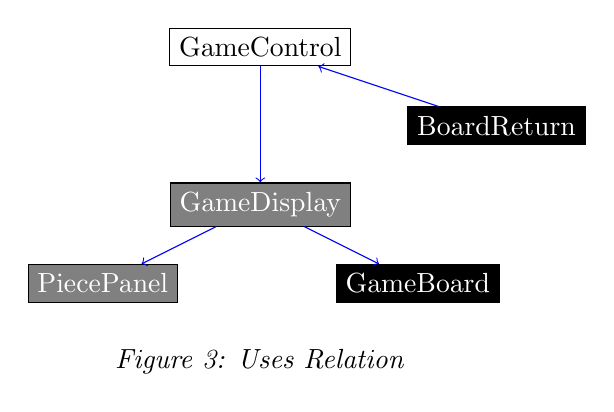
\begin{tikzpicture}
			\node[draw] (GameControl) at (1,3) {GameControl};
			\node[draw,fill=black,text=white] (GameBoard) at (3,0) {GameBoard};
			\node[draw,fill=gray,text=white] (GameDisplay) at (1,1) {GameDisplay};
			\node[draw,fill=gray,text=white] (PiecePanel) at (-1,0) {PiecePanel};
			\node[draw,fill=black,text=white] (BoardReturn) at (4,2) {BoardReturn};
			
			\draw[->,draw=blue] (GameControl) to (GameDisplay);
			\draw[->,draw=blue] (GameDisplay) to (PiecePanel);
			\draw[->,draw=blue] (GameDisplay) to (GameBoard);
			\draw[->,draw=blue] (BoardReturn) to (GameControl);
				\node at (1.0, -1.0) {\textit{Figure 3: Uses Relation}};
				
				\end{tikzpicture}
			\end{figure}
	In the above relation, a class points to another that it uses.
	The View calls the Controller, which in turn modifies the Model. In the future, the View will initially take input from the user. Then, depending on which component was clicked, will call a corresponding method in the controller. Clicking either the red or blue piece will call the newpiece method in GameControl. Clicking the check button will call checkboard(), and clicking the start button will call startboard(). These methods will then modify the model through the manipulation of arrays. \\
	\newpage	
	\section{Testing}
	% A section on the testing of the software
	%Behavoir Table
	
	\begin{tabularx}{\linewidth}{|C|C|C|}
		\hline
		What was Tested & What it did & Comments \\
		\hline \\
    GameControl: startboard & Printed out 'visibleteams' array & startboard is correctly setting up the 'visibleteams' array \\
    \hline \\
    GameControl: startboard & Printed out "first" boolean & "first" is correctly assigned random boolean values (on 3 separate tests was assigned true, false, and false) \\
    \hline \\
    GameControl: newpiece & Entered various input values (ie: 1,1,true) & Values were correctly entered into 'visibleteams' (ie: visibleteams[1][1] = 1) \\
    \hline \\
    GameControl: newpiece & Was unable to place new peices in spots already occupied (ie: visibleteams[1][1] = 1, then a newpeice was entered there) & An int value of 0 was returned (meaning the move was not legal) and the array was unchanged. \\ 
    \hline \\
    GameControl: movepiece & Ran function while no illegal moves attempted & Correctly returned no errors, updated array correctly \\
    \hline \\
    GameControl: movepiece & Attempted to move pieces illegally on top of each other (ie: piece at [0][0] moved ontop of another piece at [0][1]) & Returned 0, no changes made to 'visibleteams' array (piece remained at [0][0], no other pieces were moved) \\
    \hline \\
	\end{tabularx}
	
	\begin{tabularx}{\linewidth}{|C|C|C|}
		\hline
		What was Tested & What it did & Comments \\
		\hline \\
		 GameControl: movepiece & Attempted to move pieces illegally to positions not adjacent to the current position & Returned 0, no changes made to 'visibleteams' array (piece remained at [0][0]) \\    
		 \hline \\
		GameBoard: GameBoard() & Display the board, allow for color change of disks & Constructor Method for the gameboard panel. Displays the board as a set of pieces. \\
		\hline
		GameBoard: GameBoard() Change Piece Color& Pieces Change color & The display was successfully able to read in the current color array. \\
		\hline
	
		GameDisplay: GameDisplay() & Displayed panel in correct position in frame with buttons in correct positions in panel & GameDisplay is correctly setting up the panel \\
		\hline
		GameDisplay: GameDisplay()& Clicked on "New Game?" Button,  printed "New Game!" in command line & GameDisplay is correctly running through correct output for the given input \\
		\hline
		GameDisplay: GameDisplay() & Clicked on "Check!" Button, printed "Is is correct?" in command line & GameDisplay is correctly running through corect output for the given input \\
		\hline
		PiecePanel: PiecePanel() & Displayed panel in correct position in frame with circle tokens in correct position in panel & PiecePanel is correctly setting up the panel \\
		\hline
	\end{tabularx}
	\newpage
	\begin{tabularx}{\linewidth}{|C|C|C|}
		\hline
		What was Tested & What it did & Comments \\
		\hline 
		PiecePanel: PiecePanel() & Clicked on Red Circle, Displayed "add red?" & PiecePanel is giving the correct output for the given input and is ready to add a red piece to the board \\
		\hline
		PiecePanel: PiecePanel() &  Clicked on Blue Circle, Displayed "add blue?" & PiecePanel is giving the corect output for the given input and is ready to add a blue piece to the board \\
		\hline
		PiecePanel: PiecePanel()  , Clicked on Red Circle, then white circle & White Cirtcle turned red & PiecePanel is giving the corect output for the given input and should add a red piece to the board \\
		\hline
		PiecePanel: PiecePanel()  , Clicked on Red Circle, then white circle that has been coloured red & No output occurred & PiecePanel is giving the corect output for the given input and any additional red peices were not added not on their turn \\
		\hline
		PiecePanel: PiecePanel()  , Clicked on Blue Circle, then white circle that has been coloured red & The red coloured white circle turned blue & PiecePanel is giving the corect output for the given input and a blue piece should be added \\
		\hline
		PiecePanel: PiecePanel()  , Clicked on Blue Circle, then white circle & White Circle turned Blue & PiecePanel is giving the corect output for the given input and should add a blue piece to the board \\
		\hline
		PiecePanel: PiecePanel()  , Clicked on Blue Circle, then white circle that has been coloured blue & No output occurred & PiecePanel is giving the corect output for the given input and any additional red peices were not added not on their turn \\
		\hline
	\end{tabularx}
	\newpage
	\begin{tabularx}{\linewidth}{|C|C|C|}
		\hline
		What was Tested & What it did & Comments \\
		\hline 
		PiecePanel: PiecePanel()  , Clicked on Red Circle, then white circle that has been coloured blue & The blue coloured white circle turned red & PiecePanel is giving the corect output for the given input and a red piece should be added \\
		\hline
		GameDisplay & Attempted to add pieces to board & Pieces were added correctly. Game state (adding pieces) was displayed until each player had 6 pieces on board, turn system working correctly, and current turn was displayed. It was not possible to add pieces on top of each other. \\
		\hline
		GameDisplay & Attempted to move pieces across board & Pieces were only able to move to legal positions (adjacent), no flying was possible. Which players turn it was and when a piece was selected were displayed. \\
		\hline
		GameDisplay & Attempted to mill & When pieces were milled, state was displayed. Successfully deleted other players piece when mill formed. Game continued to function thereafter.\\ 
		\hline
		\end{tabularx}
		\newpage
		\begin{tabularx}{\linewidth}{|C|C|C|}
		\hline
		What was Tested & What it did & Comments \\
		\hline
		GameDisplay & Attempted to win game & When player is down to 2 pieces, the other player's winning status is displayed. \\
		\hline
		GameDisplay & Attempted to save and load game & Game saved and reloaded correctly, all pieces where they were left. \\  
		\hline
	\end{tabularx}
	\section{Discussion}
	%4.6 Internal review/ evaluation of design
	The design follows the MVC format very roughly. As it currently stands, the Model, View, and Controller are all spread across the same few classes: the Model is implemented in GameControl; the View is implemented in GameBoard, PiecePanel, and GameDisplay; and the Controller is implemented in GameDisplay. Each class, particularly GameDisplay, is doing much more than it should. Future iterations will have more modularized code, with features such as saving and loading being within their own class. If asked to judge the program, the group would give it a 7.5/10.
	\subsection{Anticipated Changes}
	% what was designed in anticipation of changes
	\begin{itemize}
	\item    GameControl: Will be able to track previous movements of pieces in the 'visibleteams' array (at present, can only add new pieces in and move them around). Arrays were designed to contain variables that could be modified in the future to reflect these changes. This could be used to implement the behavior of the AI in future projects. 
	In the future, the GameControl could be easily used with different dimensions (ie: 8 Men's Morris).  
	\item    Boardreturn: Class designed to hold variables needed to determine whether a move/new piece is legal. Returns a integer indicating the legality, and a int[][], indicating the current board array. Due to the design of a separate type to bundle this data, if any other data feedback is required in the future, it will be simple to add it in.
	\end{itemize}
	
\end{document}